\section{Contextualiza��o}
\label{sec:restricao}

O contexto dessa tese prev� o cen�rio de manuten��o com o uso de realidade aumentada como uma ferramenta
 para aux�lio nas tarefas rotineiras. Algumas vari�veis devem ser
 consideradas para garantir a viabilidade de implanta��o da abordagem:
\begin{itemize}
\item Velocidade de reconhecimento;
\item Qualidade do reconhecimento;
\item Invari�ncia � par�metros ambientais.
\end{itemize}


\section{Vari�veis de contorno}
\label{sec:variaveiscontorno}
O cen�rio de reconhecimento de objetos dentro da aeronave traz alguns desafios que devem ser contornados
\begin{itemize}
\item Pouca ilumina��o em ambientes internos
\item Objetos muito parecidos entre si
\item Alguns objetos com textura
\item Objeto brilhante
\end{itemize}
\section{Cen�rio}

O uso da realidade aumentada em manuten��o de aeronaves pode trazer ganho no que
tange fornecer informa��es de procedimentos ao mec�nico ou mesmo previs�o de
falhas ou reconhecimento de regi�es com falha.

 Como caso de uso ser� adotado a janela de inspe��o frontal como mostrado na
 imagem~\ref{fig:ERJ190} que mostra onde fica localizado na aeronave Embraer
 190. 
 
\begin{figure}[h!]
\centering
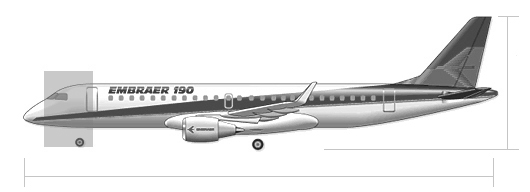
\includegraphics[scale=0.8]{images/ERJ190}
\caption{Posicionamento da LRU}
\label{fig:ERJ190}
\end{figure}


Foi selecionado um objeto sem texturas e com material brilhante como mostrado na
imagem~\ref{fig:LRU} por sofrer mais influ�ncia em varia��o de ilumina��o e ser
�nico na janela de inspe��o em quest�o.

\begin{figure}[h!]
\centering
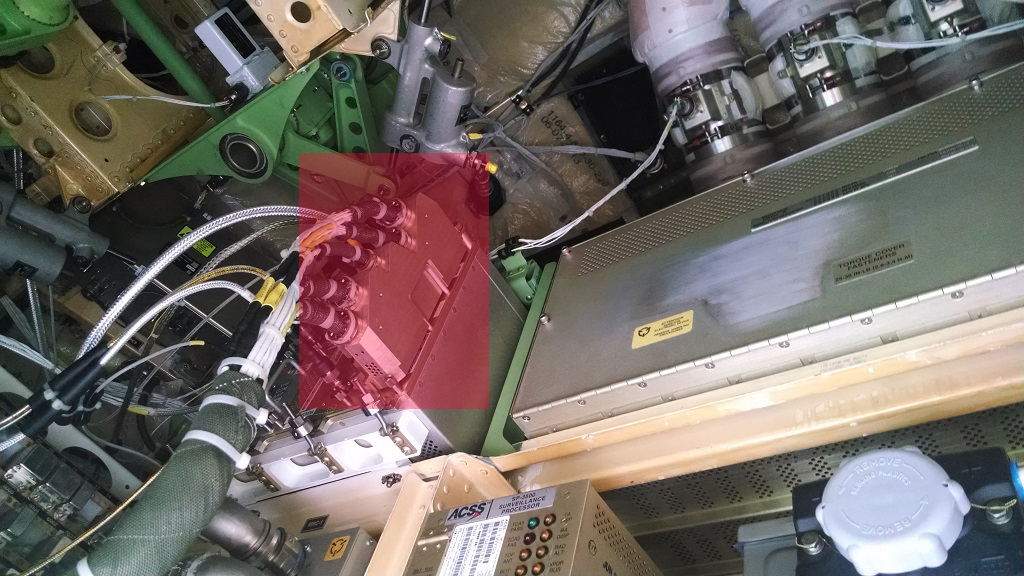
\includegraphics[scale=0.4]{images/LRU}
\caption{Imagem da LRU}
\label{fig:LRU}
\end{figure}

 


 %\section{Caso de uso}